
% !TeX spellcheck = de_DE
\documentclass{article}

\usepackage[ngerman]{babel}
\usepackage{graphicx}
\usepackage{float}
\usepackage{booktabs}
\usepackage{lscape}
\usepackage{longtable}
\usepackage{geometry}
\usepackage{caption}
\usepackage{subcaption}
\usepackage{hyperref}

\graphicspath{ {./images/} }
\setlength\parindent{0pt}

\setlength\LTleft{0pt}
\setlength\LTright{0pt}

\makeatletter
\newcommand{\sectionauthor}[1]{
	{\parindent 0em \large \scshape Autor: #1 \par \nobreak \vspace*{1em}}
	\@afterheading
}
\newcommand{\specification}[3]{
	{\parindent 0.5em \hangindent 3em \hypertarget{spec:#1:#2}{\textbf{/#1#2/}} #3 \par \nobreak \vspace*{0.5em}}
}
\makeatother

\title{BiBi - Validierungsbericht}
\date{\today\\v1.0}
\author{
	Ivan Charviakou\\
	León Liehr\\
	Jonas Picker\\
	Sergei Pravdin
}

\begin{document}

%--Titel----------------------------------------------------------------------------------------------------------------------------------------------------------------------------------
\maketitle
\begin{figure}[H]
	\centering
	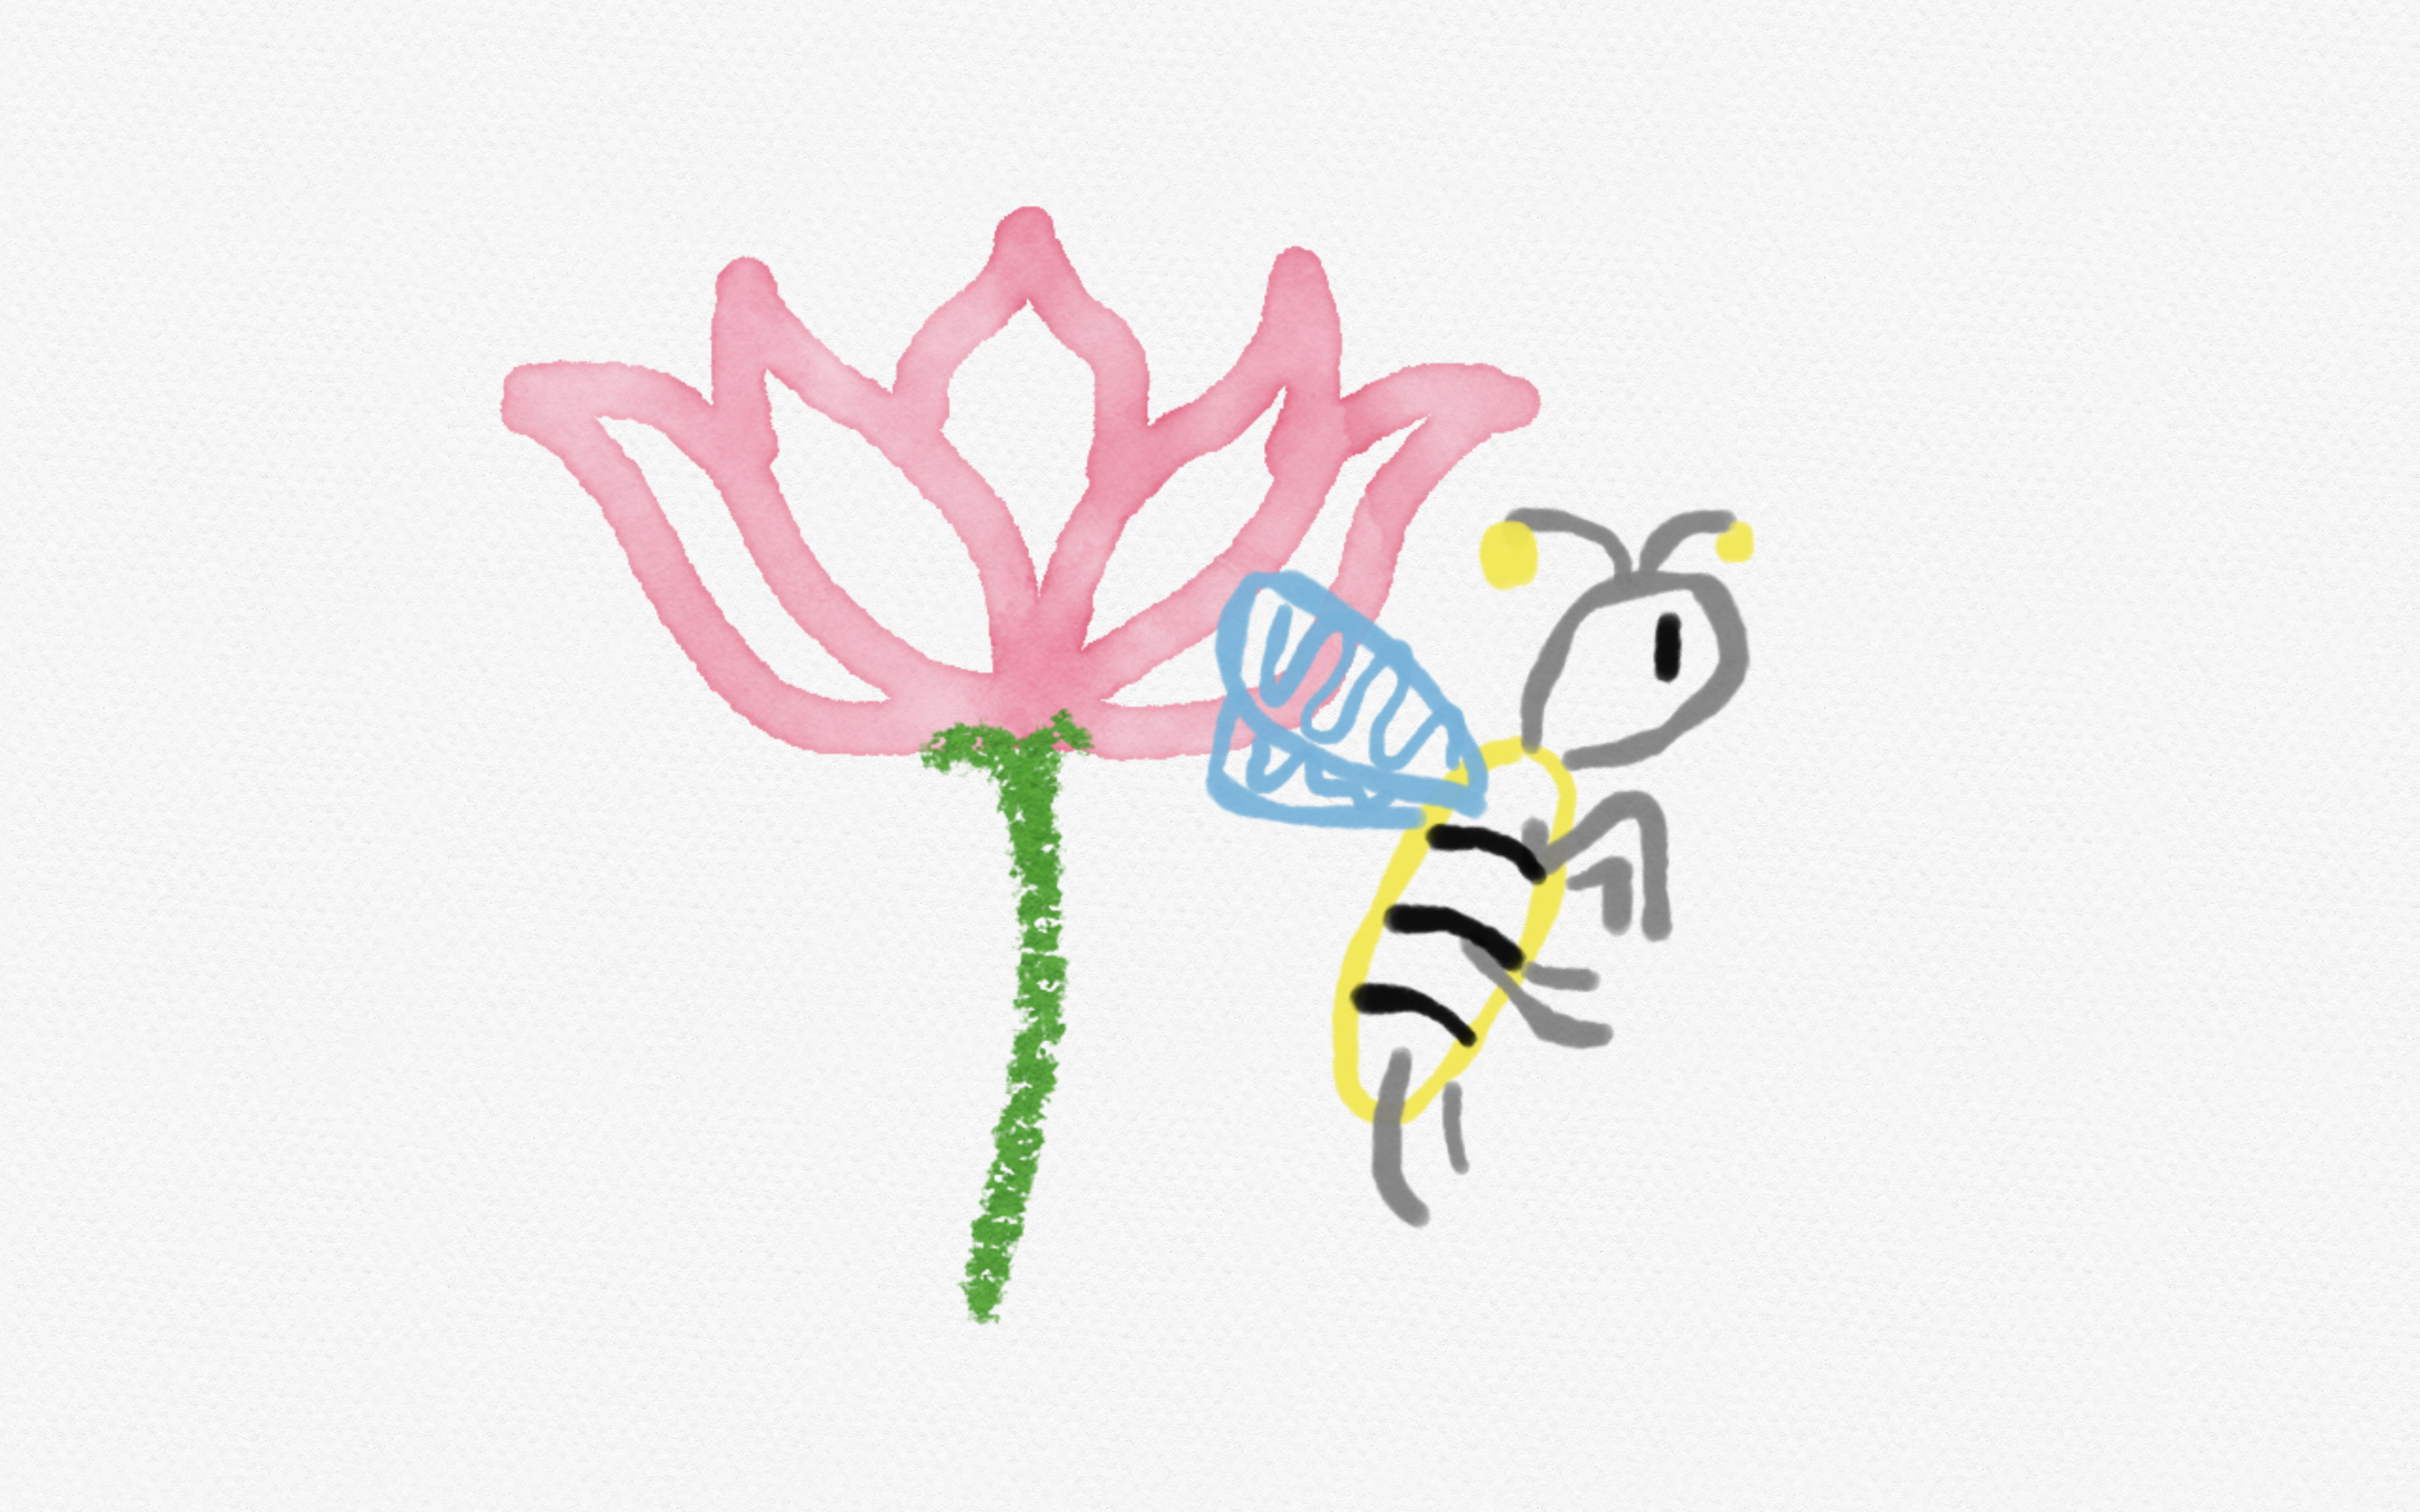
\includegraphics[width = 30em]{Logo}
\end{figure}
\newpage
\tableofcontents
\newpage

%--Einleitung--------------------------------------------------------------------------------------------------------------------------------------------------------------------------
\section{Einleitung}
\sectionauthor{Sergei Pravdin}
In diesem Dokument ist der Validierungsbericht der Webanwendung \textbf{BiBi} dokumentiert. Dabei erfolgt die \textbf{Änderungen der Tests gegenüber dem Pflichtenheft}. Außerdem sind die \textbf{Zusätzliche Tests}, die \textbf{Testergebnisse} und die \textbf{Überdeckungswerte} zu sehen.


%--Änderungen-----------------------------------------------------------------------------------------------------------------------------------------------------------------------
\section{Änderungen gegenüber dem Pflichtenheft}
\sectionauthor{Sergei Pravdin}

Seit der Erstellung des Pflichtenheftes wurde das System modifizert. Aufgrund kleinerer Änderungen, wie z.B. einer komfortableren Navigation im System, sowie anders benannten Seiten oder Abschnitten, wurden auch die Testfälle aktualisiert. Einige Tests sind irrelevant, da die Aufgabe reduziert wurde. Es wurden jedoch neue Tests für Sicherheitstests sowie ein Datenbank-Cleaner hinzugefügt, der alle von den Tests erzeugten Objekte entfernt.

\newgeometry{left=0cm,right=0cm,top=0cm,bottom=2cm}
\begin{figure}[h]
    \centering
    \includegraphics{tab1-1}
\end{figure}
\restoregeometry

\newpage

\newgeometry{left=0cm,right=0cm,top=0cm,bottom=2cm}
\begin{figure}[h]
    \centering
    \includegraphics{tab1-2}
\end{figure}
\restoregeometry

\newpage

%--Zusatztests-------------------------------------------------------------------------------------------------------------------------------------------------------------------------
\section{Zusätzliche Tests}
\sectionauthor{Jonas Picker}
\subsection{HTML-Outputvalidierung}
Aus dem Facelet-Code unserer Anwendung wird vom JSF-Framework beim Endnutzer anzeigbarer HTML-Code generiert. Dieser wurde im Zuge der Validierung mithilfe des Frameworks unter  \url{https://validator.w3.org/} auf Fehler und Stilbrüche geprüft. Da unterschiedliche Browser verschieden tolerant gegenüber fehlerhaftem HTML-Code sind, resultierten diese Fehler nicht zwingend in falschen Anzeigen und wurden so beim Implementieren übersehen. Einige Warnungen und Fehler sind JSF-internen Prozessen beim Generieren des Outputs geschuldet und außerhalb unserer Kontrolle. Darunter fallen unter anderem:
\begin{itemize}
\item Generieren des obsoleten Attributes \texttt{type='text/javascript'} innerhalb des HTML-Elements \texttt{<script/>} führt zu Warnung.
\item Setzen des Attributes \texttt{name} auf den gleichen Wert des im Facelet-Code angegebenen und ebenfalls im HTML-Code präsenten Attributes \texttt{id} in verschiedensten HTML-Elementen führt zu Warnung.
\item Automatisches Setzen des Attributs \texttt{type='hidden'} des HTML-Elements \texttt{<input/>} führt zu Errors bei referenzierenden labels und anderen Elementen mit Attribut \texttt{for}, die sich mit den Attributoptionen im korrespondierenden Facelet-Element \texttt{h:form} nicht verhindern lassen.
\end{itemize}
Es folgt eine kurze Auflistung der wichtigsten gefundenen (und verbesserten) Fehler im Zuge der Validierung:
\begin{itemize}
\item `element inside span'-Error, aufgetreten durch ein fehlendes Attribut \texttt{layout='block'} in Facelet-Elementen vom Typ \texttt{h:panelGroup} bei der Umschließung von nicht-Text-Inhalten an vielen Stellen.
\item Fehlende Deklaration des Attributes \texttt{lang} im führenden \texttt{html} Start-Tag auf allen Seiten.
\end{itemize}
\subsection{Belastungstest des Systems}
Durch die Automatisierung der Browserinteraktion mittels Selenium, diente die von uns erstellte TestSuite ebenfalls als Grundlage für die Belastungstests. Da sie in der vorherigen Phase bereits erfolgreich durchgelaufen sind, benutzen wir sie nun als Simulation einer Benutzerinteraktion. Hierbei ist zu beachten, dass diese Inputs mit maschineller Präzision ablaufen und deshalb weitaus schneller als ein normaler Mensch mit dem System interagieren. Im Zuge des Belastungstests wurde das System auf der Referenzplattform aufgesetzt und aus dem gleichen Netzwerk von einem Client-Rechner mit annähernd gleicher Hardware gleichzeitig mit XXX Threads der TestSuite belastet. Als Metrik für die Leistung dient hier die durchschnittliche Zeit zwischen Anfrage und Antwort an den Serverrechner. Diese wurde als Mittel über alle Threads errechnet, in denen die künstlichen Wartezeiten von der gesamten Durchlaufzeit einer TestSuite abgezogen, und durch die Anzahl der Anfragen geteilt wurde. Da die kurze Zeitspanne, die der WebDriver zum Befüllen der Formulare und Anklicken der Knöpfe braucht, sowie die Aufbauzeiten der Seite im Browser nicht abgezogen werden, stellt unser Wert eine obere Schranke der durchschnittlichen Request-Response-Zeit dar.

\newpage

%--Testergebnisse--------------------------------------------------------------------------------------------------------------------------------------------------------------------
\section{Testergebnisse}
\sectionauthor{León Liehr}



\newpage

%--Überdeckungswerte--------------------------------------------------------------------------------------------------------------------------------------------------------------
\section{Überdeckungswerte}
\sectionauthor{Ivan Charviakou}

Im Folgenden werden die Überdeckungswerte des Test-Suites tabellarisch angegeben und anschließend interpretiert. 
Insbesondere werden diese Werte in zwei Kategorien eingeordnet: Zur Anweisungsüberdeckung gehörend und zur Zweigüberdeckung gehörend. 
Während die Anweisungsüberdeckung die Anzahl an evaluierten Anweisungen misst, beachtet die Zweigüberdeckung die verfolgten Ausführungspfade im Kontrollflussgraphen des Programms.
Somit impliziert eine komplette Zweigüberdeckung eine höhere Anweisungsüberdeckung. 
Allerdings sind beide Werte notwendig, um die Vollständigkeit eines Test-Suites zu evaluieren.

\subsection{Whitebox-Tests}

\subsection{Blackbox-Tests}

\subsection{Alle Tests}

\subsection{Interpretation}

\newpage

%--Reference---------------------------------------------------------------------------------------------------------------------------------------------------------------------------
\section{Reference}
\sectionauthor{Wario}

\subsection{Nice looking table}
\begin{longtable}{@{}lllll@{}}
\toprule
\textbf{Header 1} & \textbf{Header 2} & \textbf{Header 3} & \textbf{Header 4} & \textbf{Header 5} \\* \midrule
\endfirsthead
%
\endhead
%
Text 1            & Text 2            & Text 3            & Text 4            & Text 5            \\
Text 1            & Text 2            & Text 3            & Text 4            & Text 5            \\* \bottomrule
\end{longtable}

\subsection{Nice looking landscape-table}
\begin{landscape}
\begin{longtable}{@{}lllll@{}}
\toprule
\textbf{Header 1} & \textbf{Header 2} & \textbf{Header 3} & \textbf{Header 4} & \textbf{Header 5} \\* \midrule
\endfirsthead
%
\endhead
%
Text 1            & Text 2            & Text 3            & Text 4            & Text 5            \\
Text 1            & Text 2            & Text 3            & Text 4            & Text 5            \\* \bottomrule
\end{longtable}
\end{landscape}

\newpage

\end{document}


